\documentclass[letterpaper,12pt]{article}
\usepackage[margin=1in]{geometry}
\usepackage{listings}
\usepackage{graphicx}
\title{Kevin Zheng's (CoffeeVector) dotfiles}
\author{Kevin Zheng}
\begin{document}
\maketitle
\tableofcontents
\section{.Xresources and .Xresources.d/}
\subsection{Introduction to the purpose of a .Xresources file}
\par The .Xresources file (previously known as the .Xdefaults file) is a file that specifies stylizations of programs.
While this does not stylize all programs, you should feel blessed when you find out a program has Xresources compatibility.
Xresources is how you can achieve the same stylization for most programs.
Most notably, the color scheme.
\par Note that after you edit the .Xresources file, it does not automatically update the system's stylization.
To update the system's stylization, you must run the command
\begin{center}
	\$ xrdb ~/.Xresources
\end{center}
\subsection{My .Xresources specifically}
\par For my .Xresources, you will first notice that it has many includes at the top which refer to a directory called .Xresources.d.
As far as I know, this is not exactly standard usage, but I prefer to keep the stylizations of different programs separate.
\par Ignoring the includes for now, you will find that the rest of the file is simply one line, which is \lstinline{Xft.dpi: 192}.
This is to ensure that everything looks as normal on a 4k screen.
If you do not have a 4k screen, you should delete this file unless if you are near sighted.
\subsubsection{theme.txt}
\par The theme.txt file is a modified .Xresources export from terminal.sexy.
It's simply a list of hexadecimal colors.
If you are in the lookout for a better colorscheme, I highly recommend that you checkout that url.
\subsubsection{color}
\par The color file simply assigns all the color attributes to the various hexidecimal colors that we have specified in theme.txt.
The first thought you may have had is ``wHy d1Dn't y0U jUSt d3clar3 tH4 c0loRs iN th1S f1l3??!? btw, i use arch linx''.
See, this is why you're reading the documentation you failure of a programmer.
A real software engineer dedicates all his free time to ricing his Linux with blood, sweat and tears, but I understand that not everyone can be competent.
Anyways, the reason why we don't declare the colors in this file is because we want to use the hexadecimal values in other files too.
If we simply declare them in this file, we can't assign other values these colors.
\subsubsection{urxvt (short for rxvt-unicode)}
\par urxvt is a terminal-emulator (not to be confused with the terminal shell such as bash or zsh).
This use to be my personal favorite except I chose to switch to st recently.
\par urxvt looks horrendous out of the box.
\begin{center}
	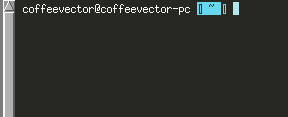
\includegraphics[width=10cm]{./images/urxvtPreXresources.png}
\end{center}
The .Xresources stylizes it such that it doesn't look like a oblong potato.
\begin{center}
	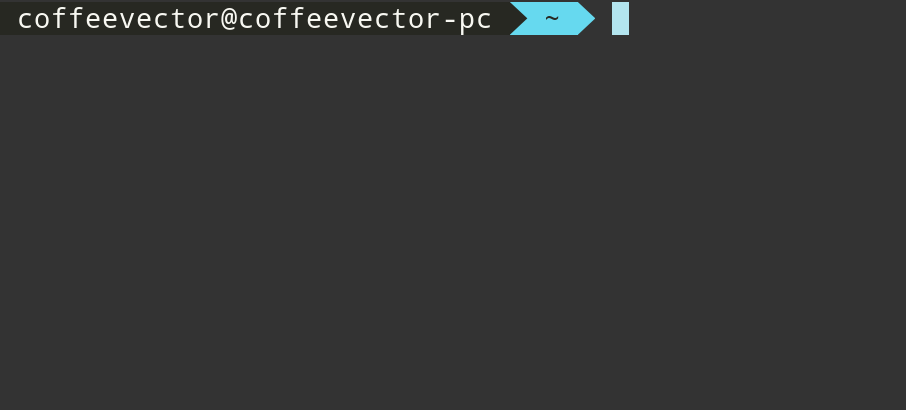
\includegraphics[width=10cm]{./images/urxvtPostXresources.png}
\end{center}
The stylizations include changing the font, changing the letter spacing, adding transparency, changing the background color, removing the scrollbar, and adding the ability to click links.
Note that the font and letter spacing are dependant on the fact that my computer runs 4k.
Feel free to change those numbers.
\subsubsection{rofi}
https://github.com/DaveDavenport/rofi
\par rofi is described as a window switcher, application launcher, and dmenu replacement.
Refer to section \ref{dmenu} for more about what dmenu exactly is.
\par Currently, there is an issue that not all the colors are properly described using the theme.txt definitions because I preferred have a certain amount of transparency.
\subsubsection{st}
\par st is my preferred terminal.
The st file only contains one line which specifies the shell.
\section{zsh \& oh-my-zsh}
https://github.com/robbyrussell/oh-my-zsh
\par zsh is a shell very similar to bash.
It includes mild differences such as being able to do
\begin{center}
	\$ cd ...
\end{center}
which changes to the parent's parent's directory.
\par While these difference(s) are kinda cool, that's not the reason why I changed to this shell.
The reason why I changed to this shell is because of oh-my-zsh which is a kind of themer for zsh.
After installing oh-my-zsh, I recommend immediately changing the them to \emph{agnoster}.
oh-my-zsh gives you interesting tools like telling you the git branch that you're in, telling you if you have unstaged/uncommitted changes.
\begin{center}
	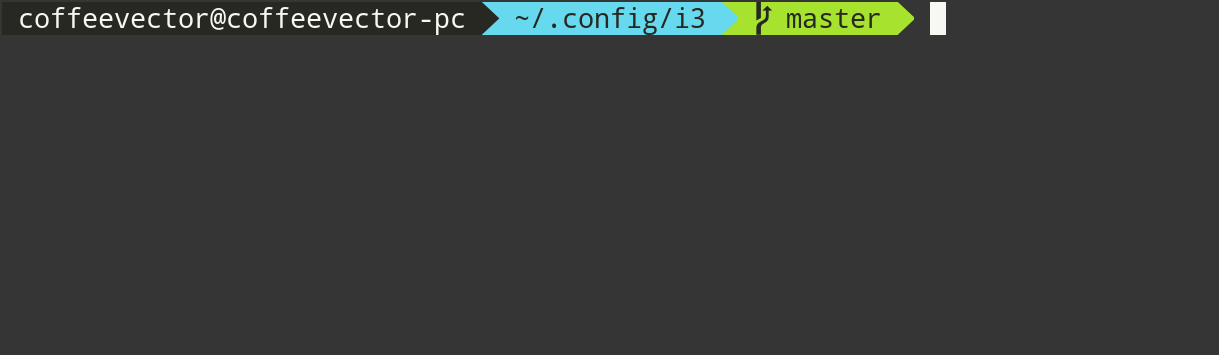
\includegraphics[width=10cm]{./images/zsh.png}
\end{center}
\section{dmenu/rofi}\label{dmenu}
\par dmenu is a general purpose menu/ui.
You pipe in the output of some bash command, and you pipe whatever you typed in to another command.
\subsection{Interesting use cases}
\subsubsection{Passwords}
\par Yes, there is a flag for you type in a password (-password).
This has been used to handle the password that I type in to access my encrypted backups.
Note that you should also add the flag ``-lines 0'' because there shouldn't be options for your password.
\subsubsection{Not typing in the given options}
\par In the .config/i3/scripts/gchrome/gchrome.sh script, there are various options, but if you were to not choose any of them, it would automatically just search your request.
This implies that dmenu doesn't necessarily need to output the options piped in.
\section{restic backup}
https://restic.net/
\par restic is a program that handles backing up files.
My favorite thing about it is that it takes \emph{snapshots}.
If I backup my system every day, I can restore a specific file from a specific date in time.
\par Personally, I keep two backups, one on my external drive, and one on my google drive.
The external drive keeps data ever since the birth of my rice while my google drive only stores files from a month old.
\section{drive (command)}
https://github.com/odeke-em/drive
\par drive is a command line application for google drive.
It's similar to how git is used.
Instead of automatically syncing like how it does in windows, you must specify to push and pull certain files/directories.
\par Personally, I keep a folder called \emph{Drive} on my home directory and symlink all my important home directory folders into it.
\section{i3 window manager}
\par i3 window manager is a \emph{tiling} window manager which does two things.
First, it makes these things called workspaces which act a lot like dual monitors (or decamonitor if you will, there are 10 workspaces) which can be accessed via hotkeys.
The second thing it does is that it automatically splits your windows such that they take up the entire screen.
I feel that this is much more natural.
\par i3 window manager
\subsection{bindsym}
\par i3 window manager also handles hotkeys.
The default config only handles hotkeys for handling the behavior of the windows, but it can just as easily be made to run programs.
\section{vim}
\par vim is a text editor which places heavy emphasis on using the keyboard for everything.
\section{ranger}
\par ranger is a terminal based file explorer which also puts emphasis on using the keyboard for everything (similarly with i3 and vim).
\section{polybar}
\par polybar is a status bar that shows up at the bottom of the screen.
Personally, I like to keep the defaults of it because of how it looks.
\section{notify-send (\& notify-send.sh)}
\par notify-send is a command that sends a notification.
notify-send.sh is the same thing but has another flag that lets you change existing notifications.
\section{scripts}
\subsection{academics.sh}
\par academics.sh is a script that takes the contents of $\sim$/Academics/Current and pipes it into a could awk and sed commands and pipes it into dmenu.
Then, ranger opens up the folder that has been selected.
\subsection{backup/}
\par The backup directory contains multiple scripts which essentially makes a ui front end for the restic command using rofi/dmenu.
\subsubsection{backup.sh}
\par The backup.sh script simply echos various options for what you want restic to do into rofi, which then proceeds to run the respective script.
\subsubsection{backup-backup.sh}
\par The backup-backup.sh script does the actual backing up.
\begin{enumerate}
	\item Runs almost infinitely long notify-send.sh saying the backup is in progress.
	\item Uses rofi to pipe the password into restic and then stores the output of restic.
	\item If the output is empty, that means that you have failed to type the right password, then replaces the notification with ``BACKUP FAILED.''.
	\item If the output is not empty, that means the backup was completely successfully, then replaces the notification with ``BACKUP COMPLETE.''.
\end{enumerate}
\subsubsection{backup-forget.sh}
\par The backup-forget.sh script handles forgetting snapshots that are old.
\begin{enumerate}
	\item Uses rofi to pipe the password into restic and then stores the output of restic.
	\item If output is empty, the password was wrong.
	\item Display all the snapshots in the repository
	\item Isolate the hexadecimal number associated with the chosen snapshot.
	\item Pipe the password again to forget the snapshot.
\end{enumerate}
\subsubsection{backup-snapshots.sh}
\subsubsection{backup-prune.sh}
\subsubsection{backup-push.sh}
\par Pushes the restic backup to google drive using the drive command.
\end{document}
